% This is lnbip.tex the demonstration file of the LaTeX macro package for
% Lecture Notes in Business Information Processing from Springer-Verlag.
% It serves as a template for authors as well.
% version 1.0 for LaTeX2e
%
\documentclass[lnbip]{svmultln}
%
\usepackage{makeidx}  % allows for indexgeneration
% \makeindex          % be prepared for an author index
%

\usepackage{color}
\usepackage{amsmath}
\usepackage{amsfonts}
\usepackage{amssymb}
\usepackage{graphicx}
%\usepackage{amsthm}
\usepackage{epsfig} 
\usepackage{lipsum}
\usepackage{float}
\usepackage{pdfpages}
\usepackage{wrapfig}
\usepackage{graphicx} 
\usepackage{subfig}  

\usepackage{chngcntr}
\counterwithin{table}{section}


\newcommand{\myfloatalign}{\centering}

\setlength{\textheight}{19.5 cm}
\setlength{\textwidth}{13.5 cm}

\setlength\parindent{0pt}

%\numberwithin{table}{section}



\begin{document}
%
\mainmatter              % start of the contribution
%
\title{Minimization of learning errors: case of invariance of geometric transformations in license plate recognition}
%
\titlerunning{Minimization of learning errors}  % abbreviated title (for running head)
%                                     also used for the TOC unless
%                                     \toctitle is used
%
\author{Hassan T. Kajila\inst{1} \and Jordan Masakuna\inst{2} \and
Pascal Sungu \and Godwill Ilunga  }
%
\authorrunning{Hassan Kajila et al.}   % abbreviated author list (for running head)
%
%%%% list of authors for the TOC (use if author list has to be modified)
\tocauthor{Hassan Kajila, Jordan Masakuna, Pascal Sungu, Godwill Ilunga}
%
\institute{Université Nouveaux Horizons, Département des Sciences Informatiques, Lubumbashi, DR Congo,\\
	\email{infos@unhorizons.org},\\ home page:
	\texttt{https://www.unhorizons.org/}
	\and
	Université de Kinshasa, Département des Sciences Informatiques, Kinshasa,\\ DR Congo}
\maketitle              % typeset the title of the contribution
% \index{Ekeland, Ivar} % entries for the author index
% \index{Temam, Roger}  % of the whole volume
% \index{Dean, Jeffrey}

\begin{abstract}        % give a summary of your paper
	Nowadays, a huge number of cameras are deployed exclusively for surveillance. The contents of images and videos are often interpreted by human operators. This makes content tracking and analysis prohibitively expensive, not to mention the mistakes that human fatigue and carelessness can introduce.
	
	This work aims to propose a method, based on artificial intelligence, which allows computer systems to derive meaningful information from digital images, with the lowest possible cost. As part of this work, the aim is to perform automatic license plate recognition using optimizers based on stochastic gradient descent.
	
	Therefore, the main objective of this present study is to examine the different optimizers, finally to determine the best able to recognize license plates, despite possible geometric transformations. In order to reduce the constraints in the detection of license plates as to the position of the camera.
	
	Experiments on several license plates that undergo a slight geometric transformation, in image, made it possible to validate the performance obtained with this approach.
%                         please supply keywords within your abstract
\keywords{Supervised learning, Optimisation, Stochastic gradient descent, Visual Geometry Group (VGG), Automatic License Plate Recognition, Invariance of geometric transformations.}
\end{abstract}

%
\section{Introduction}
%
	In this paper, it is a question of approaching the use of the algorithms of numerical optimization, precisely of minimization of the errors. They will be applied to machine learning that will allow computers and computer systems to derive meaningful information from digital images.
	
	Indeed, it is the recognition of vehicle license plates using a classifier and optimizers of the family of stochastic gradient descent implemented in a convolutional neural network (CNN). The result obtained will be used to measure the efficiency of the optimizers with respect to the constraint of invariance to the geometric transformations.\\
	Therefore for each algorithm, the efficiency of geometric transformation invariance will be examined and compared the score (accuracy, loss) for different optimizers.




%
\section{Result \& discussion}
%	
	\subsection{CNN VGG Model }
	
	\begin{table}[H]
		\centering
		\begin{tabular}{lll}
			\hline
			Layer (type) & Output Shape & Param \# \\
			\hline
			\hline
			%& & \\
			\texttt{vgg16 (Functional) } &  \texttt{(None, 6, 6, 512) } & \texttt{14714688} \\
			
			\texttt{flatten (Flatten)}  & \texttt{(None, 18432)} & \texttt{0} \\ 
			
			\texttt{dropout (Dropout)} & \texttt{(None, 18432)} & \texttt{0} \\ 
			
			\texttt{dense (Dense)} & \texttt{(None, 256)} & \texttt{4718848 }\\
			
			\texttt{dense\_1 (Dense)} & \texttt{(None, 128)} & \texttt{32896} \\
			
			\texttt{dense\_2 (Dense)} & \texttt{(None, 64)} & \texttt{8256} \\ 
			
			\texttt{dense\_3 (Dense)} & \texttt{(None, 4)} & \texttt{260}  \\
			\hline
			\hline
			\multicolumn{3}{l}{
				\begin{tabular}{l}
					\texttt{Total params: 19,474,948} \\
					\texttt {Trainable params: 4,760,260} \\
					\texttt {Non-trainable params: 14,714,688} \\
				\end{tabular}
			}\\
			\hline
			
		\end{tabular}
		\caption[]{The information the convolutional neural network builds with VGG-16.}
		\label{tab:vgg-16}
	\end{table}
	
	\subsection{Optimizer evaluation}
	\subsubsection*{\qquad \textbullet \ \textbf{SGD}}
	The SGD optimizer minimizes the model parameter with a score of 67.5\% accuracy and about 1\% error. And on the validation data, the accuracy is 72.7\% and an error of 1.2\%. The test result reveals an error of 0.73\% and an accuracy of 79.3\%.
	
	
	\begin{table}[H]
		\centering
		\begin{tabular}{l|l|l}
			\hline
			\textbf{Training} & \textbf{Validation} & \textbf{Test} \\
			%& & \\
			\hline
			
			\texttt{loss: 0.0105} & \texttt{val loss: 0.0120} & \texttt{test loss: 0.00732} \\
			\texttt{accuracy: 0.6755} & \texttt{val accuracy: 0.7273} & \texttt{test accuracy: 0.7931} \\
			
			\hline
			
		\end{tabular}
	\end{table}
	
	\begin{figure}[H]
		\myfloatalign
		\subfloat[loss : perte]
		{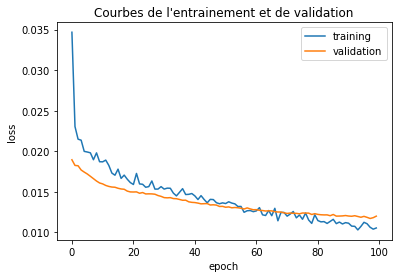
\includegraphics[width=.45\linewidth]{images/sgd_loss_curve}} \quad
		\subfloat[accuracy : précision]
		{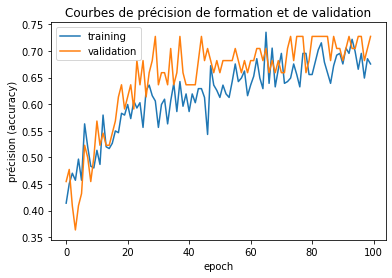
\includegraphics[width=.45\linewidth]{images/sgd_accuracy_curve}} 
		
		\caption{Accuracy and loss graph for SGD.}
	\end{figure}

	
	\subsubsection*{\qquad \textbullet \ \textbf{RMSprop}}
	
	The model minimized with the RMSprop gives a score of 95.7\% accuracy, displays a deviation of about 28.2\% compared to the SGD, and 0.044\%. The error and accuracy rate of RMSpro in validation is 1\% and 77.2\% respectively. The RMSprop optimizer also shows a lower error percentage than the SGD.
	
	The convergence of RMSprop is rather accentuated because the minimization stabilizes after 80 steps and reaches the minimum value at the 110th step.
	\begin{table}[H]
		\centering
		\begin{tabular}{l|l|l}
			\hline
			\textbf{Training} & \textbf{Validation} & \textbf{Test} \\
			%& & \\
			\hline
			
			\texttt{loss: 4.4475e-04} & \texttt{val loss: 0.0109} & \texttt{test loss : 0.005589} \\
			\texttt{accuracy: 0.9570} & \texttt{val accuracy: 0.7727} & \texttt{test accuracy : 0.8505} \\
			
			\hline
			
		\end{tabular}
	\end{table}
	\begin{figure}[H]
		
		\subfloat[loss : perte]
		{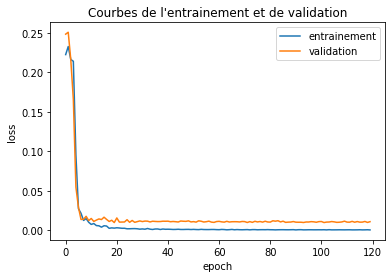
\includegraphics[width=.45\linewidth]{images/rmsprop_loss_curve}} \quad
		\subfloat[accuracy : précision]
		{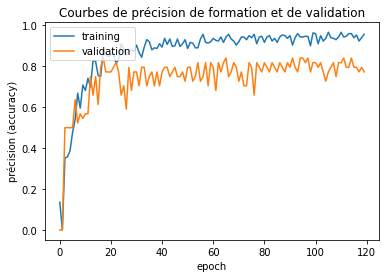
\includegraphics[width=.45\linewidth]{images/rmsprop_accuracy_curve}} 
		
		\caption{Accuracy and loss graph for RMSprop.}
		\label{fig:1}
	\end{figure}
	
	
	\subsubsection*{\qquad \textbullet \ \textbf{AdaGrad}}
	
	AdaGrad scored poorly compared to the previous optimizer, RMSprop. An error rate of 1.2\% and accuracy of 62.9\% is the score of the AdaGrad optimizer. After $120$ steps, which is the maximum step set for the tests, the minimization still does not stabilize. The minimum values are reached at the level of the $80th$ step.
	\begin{table}[H]
		\centering
		\begin{tabular}{l|l|l}
			\hline
			\textbf{Training} & \textbf{Validation} & \textbf{Test} \\
			%& & \\
			\hline
			
			\texttt{loss: 0.0124} & \texttt{val loss: 0.0156} & \texttt{test loss: 0.0094} \\
			\texttt{accuracy: 0.6291} & \texttt{val accuracy: 0.6591} & \texttt{test accuracy: 0.5747} \\
			
			\hline
			
		\end{tabular}
	\end{table}
	\begin{figure}[H]
		\myfloatalign
		\subfloat[loss : perte]
		{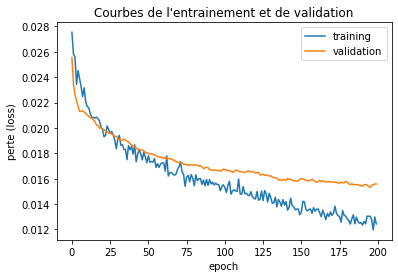
\includegraphics[width=.45\linewidth]{images/adagrad_loss_curve}} \quad
		\subfloat[accuracy : précision]
		{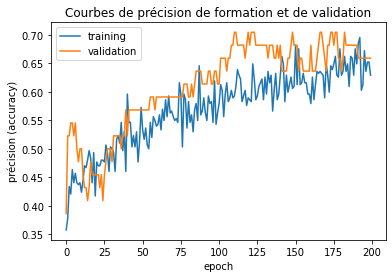
\includegraphics[width=.45\linewidth]{images/adagrad_accuracy_curve.png}} 
		
		\caption[]{Accuracy and loss graph for Adagrad.}
	\end{figure}
	
	
	\subsubsection*{\qquad \textbullet \ \textbf{Adam}}
	The Adam optimizer forms a model with 92.3\% accuracy and an error of 0.086\%, a bit higher compared to RMSprop. The validation score is 81.8\% accuracy and 1.1\% error. After the tests, 83.9\% accuracy and 0.05\% error is the observed score. RMSprop minimizes the cost better and shows a nice score compared to Adam.
	\begin{table}[H]
		\centering
		\begin{tabular}{l|l|l}
			\hline
			\textbf{Training} & \textbf{Validation} & \textbf{Test} \\
			%& & \\
			\hline
			
			\texttt{loss: 8.6163e-04} & \texttt{val loss: 0.0110} & \texttt{test loss : 0.00526} \\
			\texttt{accuracy: 0.9238} & \texttt{val accuracy: 0.8182} & \texttt{test accuracy : 0.8390} \\
			
			\hline
			
		\end{tabular}
	\end{table}
	\begin{figure}[H]
		\myfloatalign
		\subfloat[loss : perte]
		{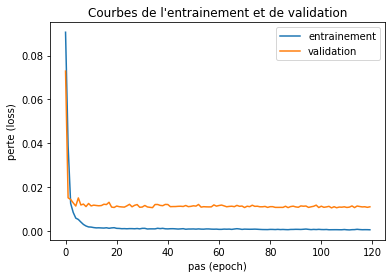
\includegraphics[width=.45\linewidth]{images/adam_loss_curve_3}} \quad
		\subfloat[accuracy : précision]
		{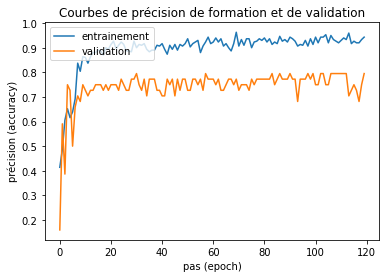
\includegraphics[width=.45\linewidth]{images/adam_accuracy_curve_3}} 
		
		\caption[]{Accuracy and loss graph for Adam.}
	\end{figure}

	
	
	\subsubsection*{\qquad \textbullet \ \textbf{Nadam}}
	Nadam, (Nesterov-accelerated Adaptive Moment Estimation), is an extension of the Adam optimizer to which we add the accelerated Nesterov gradient (NAG) \cite{ruder2016overview}.
	Nadam shows an attractive performance (from training, validation and testing point of view) compared to other optimizers studied in this work. It gives a result of 95.3\% accuracy and an error of 0.04\%. Nadam accelerates the speed of convergence in a drastic way, it stabilizes at 30 steps and reaches the minimum value in only 40 steps.
	
	\begin{table}[H]
		\centering
		\begin{tabular}{l|l|l}
			\hline
			\textbf{Training} & \textbf{Validation} & \textbf{Test} \\
			%& & \\
			\hline
			\texttt{loss: 4.6549e-04} & \texttt{val loss: 0.0109} & \texttt{test loss : 0.00479} \\
			\texttt{accuracy: 0.9536} & \texttt{val accuracy: 0.7955 }& \texttt{test accuracy : 0.9080}\\
			
			\hline 
			
		\end{tabular}
	\end{table}
	
	\begin{figure}[H]
		\myfloatalign
		\subfloat[loss : perte]
		{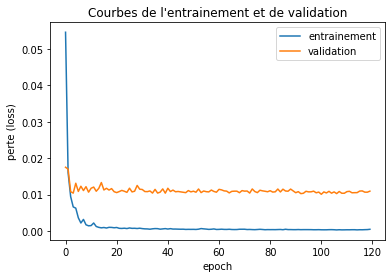
\includegraphics[width=.45\linewidth]{images/nadam_loss_curve}} \quad
		\subfloat[accuracy : précision]
		{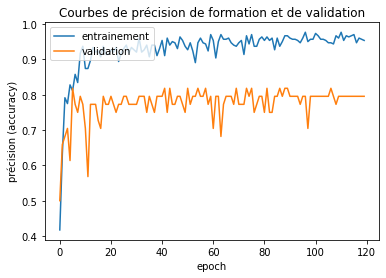
\includegraphics[width=.45\linewidth]{images/nadam_accuracy_curve}} 
		
		\caption[]{Accuracy and loss graph for Nadam}
	\end{figure}
	RMSprop gives very low error in training compared to other optimizers, in testing phase Adam reveals lower error than RMSprop. The optimizer which has a good average, in the 3 phase, is Nadam with very good precision.
	
	This work admits the Nadam optimizer as an algorithm that best minimizes errors and obtains a good score, in the context of ALPR, compared to the other optimizers studied. Below is a list of the best minimizing optimizers (table \ref{tab:error_rank}), ranked in descending order, for the case of the license plate recognition problem.
	
	
	
		\begin{table}[H]
			\centering
			\begin{tabular}{|l|p{3cm}|p{3cm}|p{3cm}|}
				\hline
				\textbf{N\textdegree} & \textbf{Training} & \textbf{Validation} & \textbf{Test} \\
				\hline
				
				\textbf{1. RMSprop} &
				\texttt{0.0004447} &
				\texttt{0.0109} &
				\texttt{0.005597} \\
				\hline
				
				\textbf{2. Nadam} &
				\texttt{0.00046549} &
				\texttt{0.0109} &
				\texttt{0.00479} \\
				\hline
				
				\textbf{3. Adam} &
				\texttt{0.00086163} &
				\texttt{0.0110} &
				\texttt{0.00526} \\
				\hline
				
				\textbf{4. Adagrad} &
				\texttt{0.0124} &
				\texttt{0.0156} &
				\texttt{0.0094} \\
				\hline
				
				\textbf{5. SGD} &
				\texttt{0.0105} &
				\texttt{0.0120} &
				\texttt{0.00732} \\
				\hline
			\end{tabular} 
		\caption{Table showing error rate per optimizer, listed in descending order. }
		\label{tab:error_rank}
		\end{table}
	
		
		The top 3 optimizers (from table \ref{tab:accuracy_rank}) served as tests in license plate detection despite the geometric transformation, i.e. the 3 models that had a good training, validation and test score.
		\begin{table}[H]
			\centering
			\begin{tabular}{l|r|r|r}
				\hline
				& \textbf{Training} & \textbf{Validation} & \textbf{Test} \\
				
				\hline
				\textbf{Nadam} &
				\texttt{95.36\%} &
				\texttt{79.55\%} &
				\texttt{90.80\%} \\
				\hline
				\textbf{Adam} &
				\texttt{92.58\%} &
				\texttt{81.82\%} &
				\texttt{83.90\%} \\
				\hline
				\textbf{RMSprop} &
				\texttt{95.70\%} &
				\texttt{77.27\%} &
				\texttt{85.05\%} \\
				\hline
				
			\end{tabular}
		\caption{Table illustrating the resulting accuracy by the 3 best optimizer.} 
		\label{tab:accuracy_rank}
		\end{table}
	
	
	
	\begin{figure}[H]%bth
		\centering
		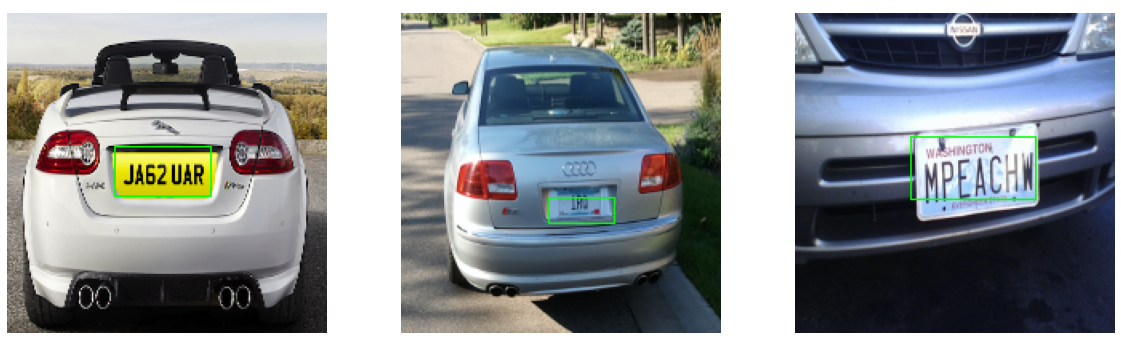
\includegraphics[width=\textwidth]{images/predicted_trans_image_2}
		%\caption{}
		\caption{The plates are recognized.}
		\label{fig:predicted_trans_image_2}
	\end{figure}

	\begin{figure}[H]%bth
		\centering
		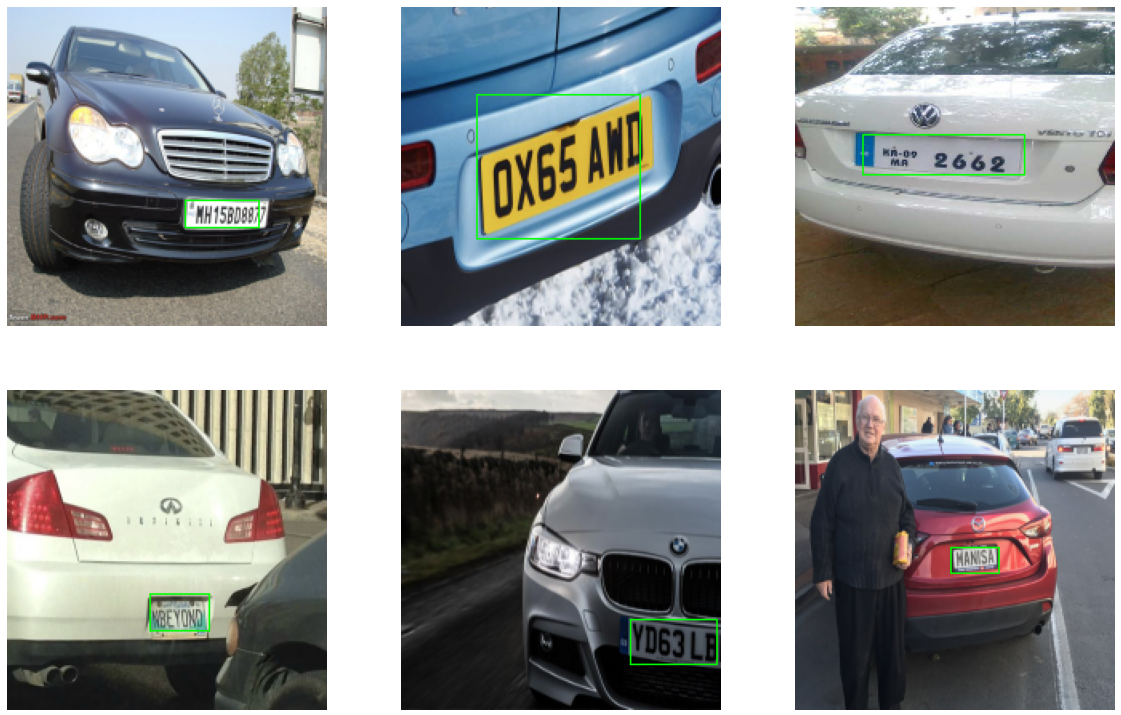
\includegraphics[width=\textwidth]{images/predicted_trans_image_1}
		\caption{The plates recognized despite the slight geometric transformation.}
		\label{fig:predicted_trans_image_1}
	\end{figure}

	With the OpenCV Python library properties, it will be easy to extract the region of interest on the image which is the detected plate in the green rectangle. OCR processing is performed on the area, as shown in figure \ref{fig:ocr_result}.

	\begin{figure}[H]%bth
		\centering
		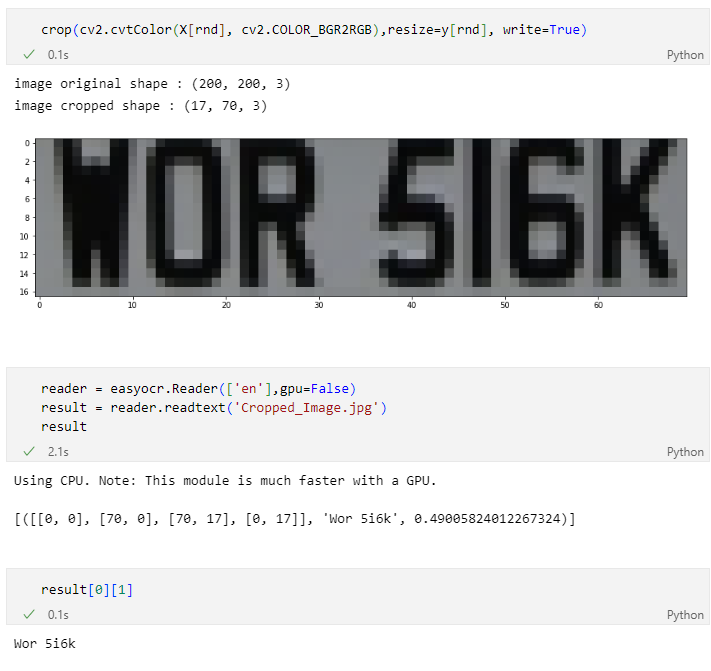
\includegraphics[width=\textwidth]{images/ocr_result_}
		%\caption{}
		\caption{The result of character recognition.}
		\label{fig:ocr_result}
	\end{figure}
	The result returned by EasyOCR Reader is an array containing a tuple of size 3, and the value we are interested in is at position 2 which corresponds to index 1 (\texttt{result[0][1]}).
	
	\texttt{result = [([[0, 0], [70, 0], [70, 17], [0, 17]], 'Wor 5i6k', 0.49005824012267324)]}
	
	The result in the \texttt{[Wor 5i6k]} terminal corresponds to the registered license plate number.
	
	



%



%
% ---- Bibliography ----
%
\bibliographystyle{plain}
\nocite{*}
\bibliography{bibliography}
%
\end{document}
